\documentclass[preview,border=4mm,convert={density=600,outext=.png}]{standalone}


\newcommand{\nodec}[3]{\node[circle,draw,minimum size=20, fill=#3] (#1#2) at (1.5*#1,1.5*#2) {};}
\newcommand{\trace}[2]{\draw[->, dotted, line width=0.1cm, red] (#1)--(#2);}

\usepackage{tikz}

\begin{document}

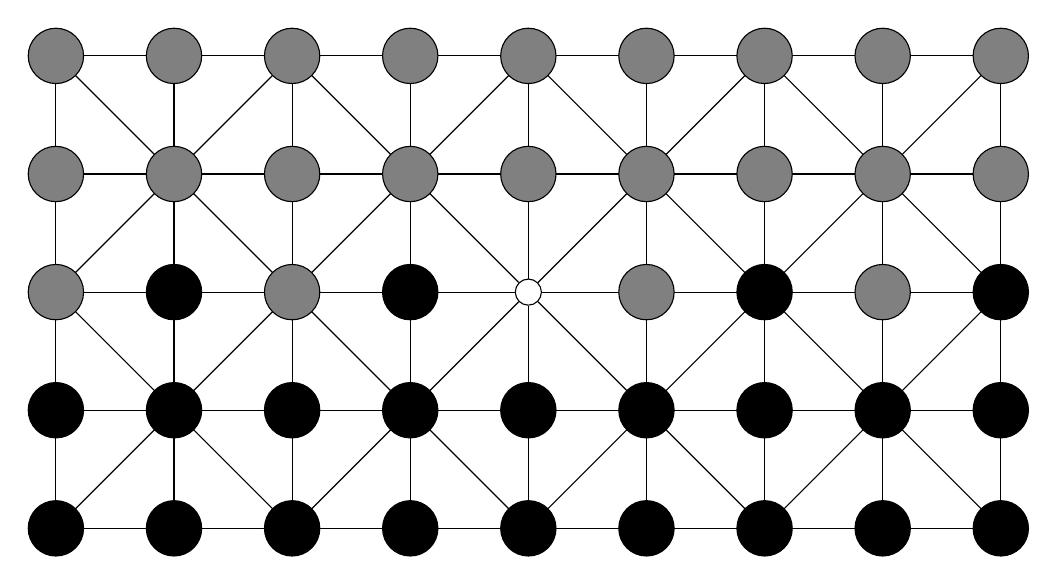
\begin{tikzpicture}
  \foreach \x in {1, ..., 9}
  \foreach \y in {1, ..., 5}
  \node[circle, draw] (\x\y) at (1.5*\x, 1.5*\y) {};

  \foreach \x [evaluate=\x as \sx using int(\x+1)] in {1, ..., 8}
    \foreach \y  in {1, ..., 5}
    \draw (\x\y)--(\sx\y);

  \foreach \y [evaluate=\y as \sy using int(\y+1)] in {1, ..., 4}
  \foreach \x in {1, ..., 9}
  \draw (\x\y)--(\x\sy);

  \foreach \x [evaluate=\x as \sx using int(\x+1),
  evaluate=\sx as \ssx using int(\sx+1)] in {1, 3, ..., 8}{
    \foreach \y [evaluate=\y as \sy using int(\y+1),
    evaluate=\sy as \ssy using int(\sy+1)] in {1, 3, ..., 4}{
      \draw (\x\y)--(\sx\sy) (\sx\sy)--(\ssx\ssy);
    }
  }
  
  \foreach \x [evaluate=\x as \px using int(\x-1),
  evaluate=\px as \ppx using int(\px-1)] in {3, 5, ..., 9}{
    \foreach \y [evaluate=\y as \sy using int(\y+1),
    evaluate=\sy as \ssy using int(\sy+1)] in {1, 3}{
      \draw (\x\y)--(\px\sy) (\px\sy)--(\ppx\ssy);
    }
  }  

  % Add players
  % -----------
  
  % Player 1
  % --------
  
  \foreach \x in {1, ..., 9}
  \foreach \y in {4, 5}
  \nodec{\x}{\y}{gray};
  
  \foreach \x in {1, 3, 6, 8}
  \nodec{\x}{3}{gray};

  % Player 2
  % -----------
  
  \foreach \x in {1, ..., 9}
  \foreach \y in {1, 2}
  \nodec{\x}{\y}{black};
  
  \foreach \x in {2, 4, 7, 9}
  \nodec{\x}{3}{black};

  % Fitaritana
  % ==========

  % Vaky Loha
  % \trace{52}{53};
  % \nodec{5}{4}{red};
  % \nodec{5}{5}{red};
  
  % Havanana
  % \trace{42}{53};
  % \nodec{6}{4}{red};
  % \nodec{7}{5}{red};

  % Havia
  % \trace{62}{53};
  % \nodec{4}{4}{red};
  % \nodec{3}{5}{red};

  % Kobaka lava
  % \trace{63}{53};
  % \nodec{7}{3}{red};

  
  % Kobaka fohy
  % \trace{63}{53};
  % \nodec{4}{3}{red};
  
  
\end{tikzpicture}
\end{document}

%%% Local Variables: 
%%% mode: latex   
%%% TeX-master: t   
%%% End: